\documentclass[11pt,a4paper]{article}

\usepackage{amsmath,amssymb}
\usepackage{booktabs}
\usepackage{graphicx}
\usepackage[margin=1in]{geometry}
\usepackage{hyperref}
\usepackage{xcolor}
\usepackage{tikz}

\title{Single Mode Ensemble PIV: Theory and Reynolds Stress Estimation}
\author{}
\date{}

\begin{document}

\maketitle

%==============================================================================
\section{Ensemble PIV Fundamentals}

\subsection{Sum of Correlation Approach}

Traditional instantaneous PIV computes a cross-correlation for each image pair independently:
\begin{equation}
    R_{AB}^{(i)}(\mathbf{r}) = A_i \star B_i
\end{equation}
where $A_i$ and $B_i$ are the first and second exposure images for the $i$-th realization.

\textbf{Ensemble PIV} instead sums correlations over $N$ image pairs:
\begin{equation}
    R_{AB}(\mathbf{r}) = \frac{1}{N} \sum_{i=1}^{N} R_{AB}^{(i)}(\mathbf{r}) = \frac{1}{N} \sum_{i=1}^{N} A_i \star B_i
\end{equation}

In Fourier space, this becomes:
\begin{equation}
    \mathcal{F}(R_{AB}) = \frac{1}{N} \sum_{i=1}^{N} \mathcal{F}(B_i) \cdot \mathcal{F}^*(A_i)
\end{equation}

\subsection{Benefits of Ensemble Averaging}

\begin{enumerate}
    \item \textbf{Improved Signal-to-Noise:} Random noise cancels while coherent signal accumulates
    \item \textbf{Smaller Interrogation Windows:} Fewer particles per window required when averaging over many realizations
    \item \textbf{Enhanced Near-Wall Resolution:} Smaller windows enable measurements closer to boundaries
    \item \textbf{Robustness:} Outliers and spurious peaks are suppressed by averaging
\end{enumerate}

\subsection{Trade-offs}

The fundamental trade-off is the \textbf{loss of time development information}:
\begin{itemize}
    \item Instantaneous PIV: $N$ independent velocity fields, temporal dynamics preserved
    \item Ensemble PIV: One averaged correlation, only statistical quantities recovered
\end{itemize}

Ensemble PIV is therefore suited for \textbf{statistically stationary} flows where we seek converged mean and turbulence statistics rather than time-resolved dynamics.

%==============================================================================
\section{Reynolds Stress Estimation from Correlation Peak Shape}

\subsection{Velocity Decomposition}

Following Reynolds decomposition, instantaneous velocities are split into mean and fluctuating components:
\begin{align}
    U_t &= \bar{U} + U'_t \\
    V_t &= \bar{V} + V'_t
\end{align}
where the overbar denotes ensemble (or time) averaging, and primes denote fluctuations.

\subsection{Correlation Peak Broadening}

In instantaneous PIV, all particles within an interrogation window move with approximately the same displacement, producing a sharp correlation peak. Over an ensemble of realizations with velocity fluctuations, particles experience a \textbf{distribution} of displacements centered on the mean.

The cross-correlation is the autocorrelation \emph{convolved} with the velocity probability density function:
\begin{equation}
    R_{AB} = R_{AA} \circledast \text{PDF}(\text{velocity})
\end{equation}

For turbulent flows with Gaussian velocity fluctuations:
\begin{equation}
    R_{AB} = R_{AA} \circledast \mathcal{N}(\boldsymbol{\mu}, \boldsymbol{\Sigma})
\end{equation}
where $\boldsymbol{\mu}$ is the mean displacement and $\boldsymbol{\Sigma}$ is the velocity covariance (Reynolds stress tensor).

\subsection{Gaussian Variance Relations}

The autocorrelation peak shape reflects only the particle image diameter:
\begin{align}
    \sigma_x^2 &= d_x^2 \\
    \sigma_y^2 &= d_y^2
\end{align}

The cross-correlation peak is broadened by velocity fluctuations:
\begin{align}
    \sigma_x^2 &= d_x^2 + \overline{u'u'} \\
    \sigma_y^2 &= d_y^2 + \overline{v'v'} \\
    \sigma_{xy} &= \overline{u'v'}
\end{align}

By comparing autocorrelation and cross-correlation peak shapes, the Reynolds stress components can be extracted:
\begin{align}
    \overline{u'u'} &= \sigma_{x,AB}^2 - \sigma_{x,AA}^2 \\
    \overline{v'v'} &= \sigma_{y,AB}^2 - \sigma_{y,AA}^2 \\
    \overline{u'v'} &= \sigma_{xy,AB}
\end{align}

%==============================================================================
\section{Single Mode: Asymmetric Window Weighting}

\subsection{The Near-Wall Resolution Problem}

Standard ensemble PIV uses symmetric windows: both Frame A and Frame B are extracted with identical interrogation regions. The measurement location corresponds to the window center, so the minimum distance to a wall is approximately half the window size. For a 64-pixel window, measurements cannot approach closer than $\sim$32 pixels from the wall.

\subsection{Single Mode Architecture}

Single mode ensemble PIV uses \textbf{asymmetric weighting} between the two frames to achieve finer spatial resolution while maintaining FFT efficiency. Three window sizes are involved:

\begin{enumerate}
    \item \textbf{Particle Window} (small, e.g., $16 \times 16$ or $8 \times 8$): The effective measurement region
    \item \textbf{Sum Window} (large, e.g., $64 \times 64$): The FFT computation size
    \item \textbf{Fitting Window} (optional, e.g., $32 \times 32$): Region extracted from correlation for Gaussian fitting
\end{enumerate}

\begin{figure}[h]
\centering
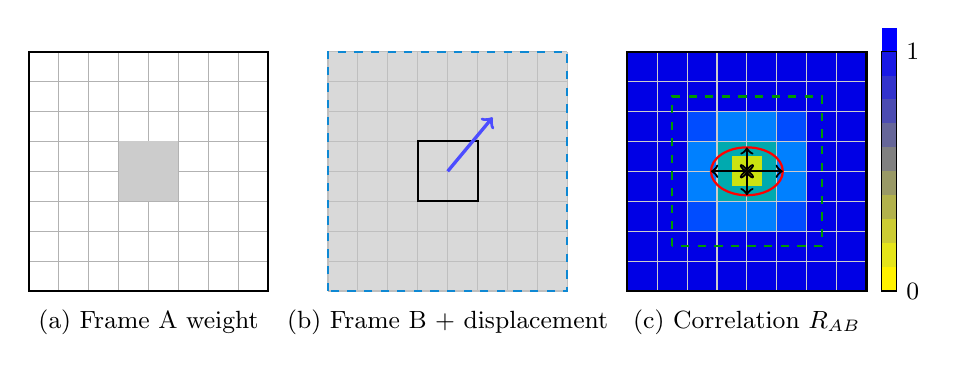
\begin{tikzpicture}[scale=0.38]
    % ===== Panel (a): Frame A weighting (singlepix) =====
    \begin{scope}[shift={(0,0)}]
        % Draw 8x8 grid
        \foreach \i in {0,...,8} {
            \draw[gray!60] (\i,0) -- (\i,8);
            \draw[gray!60] (0,\i) -- (8,\i);
        }
        % Particle window (center 2x2 region, representing small window)
        \fill[gray!40] (3,3) rectangle (5,5);
        \draw[black, thick] (0,0) rectangle (8,8);
        % Label
        \node[below] at (4,-0.3) {\small (a) Frame A weight};
    \end{scope}

    % ===== Panel (b): Frame B weighting + displacement =====
    \begin{scope}[shift={(10,0)}]
        % Full gray background (B uses full window)
        \fill[gray!30] (0,0) rectangle (8,8);
        % Draw 8x8 grid
        \foreach \i in {0,...,8} {
            \draw[gray!50] (\i,0) -- (\i,8);
            \draw[gray!50] (0,\i) -- (8,\i);
        }
        % Sum window outline (cyan dashed)
        \draw[cyan!70!blue, thick, dashed] (0,0) rectangle (8,8);
        % Particle window position in A (small box)
        \draw[black, thick] (3,3) rectangle (5,5);
        % Displacement arrow
        \draw[->, blue!70, very thick] (4,4) -- (5.5,5.8);
        % Label
        \node[below] at (4,-0.3) {\small (b) Frame B + displacement};
    \end{scope}

    % ===== Panel (c): Correlation result =====
    \begin{scope}[shift={(20,0)}]
        % Create pixelated Gaussian using nested loops
        % Background (dark blue)
        \fill[blue!90!black] (0,0) rectangle (8,8);
        % Approximate Gaussian with colored rectangles
        % Ring 4 (outermost visible)
        \foreach \x/\y in {2/2,2/3,2/4,2/5,3/2,3/5,4/2,4/5,5/2,5/3,5/4,5/5} {
            \fill[blue!70!cyan] (\x,\y) rectangle (\x+1,\y+1);
        }
        % Ring 3
        \fill[blue!50!cyan] (2,3) rectangle (3,5);
        \fill[blue!50!cyan] (5,3) rectangle (6,5);
        \fill[blue!50!cyan] (3,2) rectangle (5,3);
        \fill[blue!50!cyan] (3,5) rectangle (5,6);
        % Ring 2
        \fill[cyan!60!green] (3,3) rectangle (5,5);
        % Ring 1 (center - brightest)
        \fill[yellow!80!green] (3.5,3.5) rectangle (4.5,4.5);

        % Grid overlay
        \foreach \i in {0,...,8} {
            \draw[gray!40] (\i,0) -- (\i,8);
            \draw[gray!40] (0,\i) -- (8,\i);
        }
        \draw[black, thick] (0,0) rectangle (8,8);

        % Fitting window (green dashed) - extracted region for Gaussian fitting
        \draw[green!60!black, thick, dashed] (1.5,1.5) rectangle (6.5,6.5);

        % Ellipse showing Gaussian fit
        \draw[red, thick] (4,4) ellipse (1.2 and 0.8);
        % Arrows showing sigma
        \draw[<->, black, thick] (4,4) -- (5.2,4);
        \draw[<->, black, thick] (4,4) -- (4,4.8);
        \draw[<->, black, thick] (2.8,4) -- (4,4);
        \draw[<->, black, thick] (4,3.2) -- (4,4);

        % Colorbar
        \foreach \i in {0,...,10} {
            \pgfmathsetmacro{\col}{10*\i}
            \fill[blue!\col!yellow] (8.5,\i*0.8) rectangle (9,\i*0.8+0.8);
        }
        \draw[black] (8.5,0) rectangle (9,8);
        \node[right, font=\small] at (9,8) {1};
        \node[right, font=\small] at (9,0) {0};

        % Label
        \node[below] at (4,-0.3) {\small (c) Correlation $R_{AB}$};
    \end{scope}
\end{tikzpicture}
\caption{Single mode window weighting. (a) Frame A uses singlepix weighting: $W_A=1$ only in the small central particle window (gray), $W_A=0$ elsewhere. (b) Frame B uses uniform weighting over the full sum window (gray, cyan dashed outline); the arrow indicates particle displacement. (c) Resulting correlation plane with Gaussian peak; the green dashed line shows the fitting window region extracted for Gaussian fitting; the red ellipse and arrows indicate the fitted peak shape encoding displacement and Reynolds stresses.}
\label{fig:single_mode_windows}
\end{figure}

\subsection{The Singlepix Weighting Function}

The key to single mode is the \textbf{singlepix} weighting applied to Frame A:
\begin{equation}
    W_A(x, y) = \begin{cases}
        1 & \text{if } (x,y) \in \text{particle window (centered)} \\
        0 & \text{otherwise}
    \end{cases}
\end{equation}

Frame B uses uniform weighting over the full sum window:
\begin{equation}
    W_B(x, y) = 1 \quad \forall (x,y) \in \text{sum window}
\end{equation}

The weighted correlation becomes:
\begin{equation}
    R_{AB}(\mathbf{r}) = \mathcal{F}^{-1}\left[ \mathcal{F}(W_A \cdot A) \cdot \mathcal{F}^*(W_B \cdot B) \right]
\end{equation}

\subsection{Why Asymmetric Weighting Works}

The particle window in Frame A defines \emph{where} the measurement is localized---only particles within this small central region contribute to the correlation. The larger sum window in Frame B provides the \emph{search range} for matching displaced particles.

This asymmetry allows:
\begin{itemize}
    \item \textbf{Fine spatial resolution:} The measurement represents only the particle window region
    \item \textbf{Large displacement capture:} Particles can move anywhere within the sum window and still be matched
    \item \textbf{FFT efficiency:} Both frames are padded to the same sum window size for FFT computation
\end{itemize}

\subsection{The Fitting Window (sum\_fitting\_window)}

The full correlation plane from single mode has dimensions of the sum window (e.g., $64 \times 64$). However, Gaussian fitting only needs the central peak region. The \textbf{fitting window} extracts a smaller central portion (e.g., $32 \times 32$) for two reasons:

\begin{enumerate}
    \item \textbf{Reduced computation:} Fewer points to fit
    \item \textbf{Noise exclusion:} Correlation values far from the peak contain primarily noise
\end{enumerate}

The fitting window must be large enough to capture the full Gaussian peak shape (typically $2$--$3\times$ the expected peak width).

\subsection{Amplitude Normalization in Single Mode}

Because Frame A uses a smaller effective area than Frame B, the cross-correlation amplitude is reduced by a factor of $\sqrt{\text{particle\_area} / \text{sum\_area}}$. When validating fitted parameters, this geometric factor must be accounted for:
\begin{equation}
    R_{AB,\text{normalized}} = R_{AB} \times \sqrt{\frac{\text{sum\_area}}{\text{particle\_area}}}
\end{equation}

%==============================================================================
\section{The 13-Point Gaussian Fitting Procedure}

\subsection{Overview}

To extract mean displacement and Reynolds stresses from the ensemble correlation, we fit 2D Gaussian functions to both the autocorrelation and cross-correlation peaks. A \textbf{13-point stencil} centered on the peak maximum provides robust parameter estimation with minimal computational cost.

\subsection{Autocorrelation Fitting ($R_{AA}$, $R_{BB}$)}

The autocorrelation of each image with itself yields the particle image shape:
\begin{equation}
    R_{AA}(\mathbf{r}) = A \exp\left( -\frac{(x-x_0)^2}{2\sigma_{x,A}^2} - \frac{(y-y_0)^2}{2\sigma_{y,A}^2} \right)
\end{equation}

For symmetric particle images, $\sigma_{x,A} = \sigma_{y,A} = d_\tau$ where $d_\tau$ is the particle image diameter.

The fit extracts:
\begin{itemize}
    \item Peak location $(x_0, y_0)$ --- should be at origin for autocorrelation
    \item Widths $\sigma_{x,A}$, $\sigma_{y,A}$ --- particle image diameter
    \item Amplitude $A$
\end{itemize}

\subsection{Cross-Correlation Fitting ($R_{AB}$)}

The cross-correlation peak is fitted with a general 2D Gaussian including correlation:
\begin{equation}
    R_{AB}(\mathbf{r}) = A \exp\left( -\frac{1}{2} \begin{bmatrix} x - \mu_x \\ y - \mu_y \end{bmatrix}^T \boldsymbol{\Sigma}^{-1} \begin{bmatrix} x - \mu_x \\ y - \mu_y \end{bmatrix} \right)
\end{equation}

where the covariance matrix is:
\begin{equation}
    \boldsymbol{\Sigma} = \begin{bmatrix} \sigma_x^2 & \sigma_{xy} \\ \sigma_{xy} & \sigma_y^2 \end{bmatrix}
\end{equation}

The fit extracts:
\begin{itemize}
    \item Peak location $(\mu_x, \mu_y)$ --- mean displacement
    \item Widths $\sigma_x$, $\sigma_y$ --- combined particle + velocity variance
    \item Covariance $\sigma_{xy}$ --- related to $\overline{u'v'}$
    \item Amplitude $A$
\end{itemize}

\subsection{Joint Optimization Rationale}

Rather than fitting autocorrelation and cross-correlation independently, a \textbf{joint optimization} approach offers advantages:

\begin{enumerate}
    \item \textbf{Consistent Particle Diameter:} The same $d_\tau$ appears in both $R_{AA}$ and $R_{AB}$
    \item \textbf{Physical Constraints:} Reynolds stresses must be positive semidefinite
    \item \textbf{Reduced Parameter Count:} Shared parameters reduce degrees of freedom
    \item \textbf{Improved Robustness:} Joint fitting is less sensitive to noise in individual correlations
\end{enumerate}

The joint objective function minimizes:
\begin{equation}
    \mathcal{L} = \sum_{j=1}^{13} \left[ \left( R_{AA,j} - G_{AA}(\mathbf{r}_j; d_\tau) \right)^2 + \left( R_{AB,j} - G_{AB}(\mathbf{r}_j; \boldsymbol{\mu}, \boldsymbol{\Sigma}) \right)^2 \right]
\end{equation}

subject to the constraint that the velocity covariance $\boldsymbol{\Sigma} - d_\tau^2 \mathbf{I}$ is positive semidefinite.

%==============================================================================
\section{Ensuring Physical Validity via Cholesky Decomposition}

\subsection{The Positive Semidefinite Requirement}

A covariance matrix must be \textbf{positive semidefinite} (PSD) for physical validity:
\begin{equation}
    \mathbf{x}^T \boldsymbol{\Sigma} \mathbf{x} \geq 0 \quad \forall \mathbf{x}
\end{equation}

For the Reynolds stress tensor, this means:
\begin{itemize}
    \item Diagonal elements (normal stresses) must be non-negative: $\overline{u'u'} \geq 0$, $\overline{v'v'} \geq 0$
    \item The determinant must be non-negative: $\overline{u'u'} \cdot \overline{v'v'} \geq (\overline{u'v'})^2$
\end{itemize}

Unconstrained fitting may produce unphysical results violating these conditions.

\subsection{Cholesky Decomposition}

Any positive semidefinite matrix $\boldsymbol{\Sigma}$ can be uniquely decomposed as:
\begin{equation}
    \boldsymbol{\Sigma} = \mathbf{L} \mathbf{L}^T
\end{equation}

where $\mathbf{L}$ is a lower triangular matrix with non-negative diagonal elements:
\begin{equation}
    \mathbf{L} = \begin{bmatrix} L_{11} & 0 \\ L_{21} & L_{22} \end{bmatrix}, \quad L_{11} \geq 0, \quad L_{22} \geq 0
\end{equation}

This gives:
\begin{equation}
    \boldsymbol{\Sigma} = \begin{bmatrix} L_{11}^2 & L_{11} L_{21} \\ L_{11} L_{21} & L_{21}^2 + L_{22}^2 \end{bmatrix}
\end{equation}

\subsection{Constrained Optimization via Cholesky Parameterization}

Instead of optimizing $\boldsymbol{\Sigma}$ directly, we optimize the Cholesky factor $\mathbf{L}$:

\begin{enumerate}
    \item Parameterize: $L_{11} \geq 0$, $L_{21} \in \mathbb{R}$, $L_{22} \geq 0$
    \item Compute: $\boldsymbol{\Sigma} = \mathbf{L} \mathbf{L}^T$
    \item Evaluate: Objective function using this $\boldsymbol{\Sigma}$
\end{enumerate}

This \textbf{automatically guarantees} positive semidefiniteness without explicit inequality constraints. The optimization becomes unconstrained in $L_{21}$ and simply bounded in $L_{11}$, $L_{22}$.

\subsection{Recovering Reynolds Stresses}

From the fitted Cholesky factors:
\begin{align}
    \overline{u'u'} &= L_{11}^2 - d_\tau^2 \\
    \overline{v'v'} &= L_{21}^2 + L_{22}^2 - d_\tau^2 \\
    \overline{u'v'} &= L_{11} L_{21}
\end{align}

The particle diameter contribution $d_\tau^2$ is subtracted since it appears in both auto- and cross-correlations.

%==============================================================================
\section{Summary}

\begin{enumerate}
    \item \textbf{Ensemble PIV} sums correlations over many image pairs, trading temporal resolution for enhanced spatial resolution and statistical convergence.

    \item \textbf{Correlation peak broadening} encodes velocity fluctuation statistics: the cross-correlation is the autocorrelation convolved with the velocity PDF.

    \item \textbf{Reynolds stresses} are extracted by comparing autocorrelation and cross-correlation peak shapes:
    \begin{equation*}
        \overline{u'u'} = \sigma_{x,AB}^2 - \sigma_{x,AA}^2, \quad \overline{v'v'} = \sigma_{y,AB}^2 - \sigma_{y,AA}^2, \quad \overline{u'v'} = \sigma_{xy,AB}
    \end{equation*}

    \item \textbf{Single mode} uses asymmetric window weighting---a small particle window for Frame A embedded in a larger sum window---to achieve fine spatial resolution while preserving FFT efficiency and displacement range.

    \item \textbf{Gaussian fitting} extracts displacement and peak shape parameters; the optional fitting window reduces the correlation region used for fitting.

    \item \textbf{Cholesky parameterization} of the covariance matrix guarantees physically valid (positive semidefinite) Reynolds stress estimates during optimization.
\end{enumerate}

\end{document}
